% Neuro-Symbolic Safe Driving: a neural driver, real traffic law, and three ways to join them
% Build:    latexmk -pdf nesy_presentation.tex      (or: pdflatex nesy_presentation.tex twice)
% Charts:   python make_figures.py                  (redraws figures/*.pdf from the results in data/)
% Videos:   videos/ (mp4 + gif); they play in the repository README
\documentclass[aspectratio=169,10pt,xcolor=table]{beamer}

% ── edit these ────────────────────────────────────────────────────────────────────────────────────
\newcommand{\presenter}{Silver Gjeka}
\newcommand{\studentid}{VR527645}
\newcommand{\talktitle}{Neuro-Symbolic Safe Driving}

% ── packages ──────────────────────────────────────────────────────────────────────────────────────
\usepackage[T1]{fontenc}
\usepackage[default]{lato}
\usepackage[letterspace=120]{microtype}
\usepackage{amsmath,amssymb}
\usepackage{booktabs}
\usepackage{graphicx}
\usepackage{tcolorbox}
\usepackage{tikz}
\usetikzlibrary{arrows.meta,positioning,calc}

% ── palette (the same colours as the charts in figures/) ─────────────────────────────────────────
\definecolor{ink}{HTML}{1D1D1B}
\definecolor{ink2}{HTML}{52514E}
\definecolor{muted}{HTML}{898781}
\definecolor{hair}{HTML}{E1E0D9}
\definecolor{surface}{HTML}{F3F5F8}
\definecolor{brand}{HTML}{14284B}     % titles, dark slides
\definecolor{accent}{HTML}{EB6834}    % highlights, the winner, QR-DQN
\definecolor{cblue}{HTML}{2A78D6}     % DQN
\definecolor{caqua}{HTML}{1BAF7A}     % PPO
\definecolor{hardc}{HTML}{C62828}     % hard rules
\definecolor{softc}{HTML}{2E7D32}     % soft rules

% ── theme ─────────────────────────────────────────────────────────────────────────────────────────
\setbeamertemplate{navigation symbols}{}
\setbeamercolor{normal text}{fg=ink}
\setbeamercolor{structure}{fg=brand}
\setbeamercolor{alerted text}{fg=accent}
\setbeamercolor{caption name}{fg=muted}
\setbeamerfont{frametitle}{series=\bfseries,size=\Large}
\setbeamerfont{caption}{size=\scriptsize}
\setbeamertemplate{caption}{\centering\color{muted}\insertcaption\par}
\setbeamertemplate{itemize item}{\raisebox{0.28ex}{\color{accent}\rule{0.38em}{0.38em}}}
\setbeamertemplate{itemize subitem}{\color{muted}\textendash}
\setbeamertemplate{enumerate item}{\color{accent}\bfseries\insertenumlabel.}
\setlength{\leftmargini}{1.1em}
\setbeamertemplate{blocks}[rounded][shadow=false]
\setbeamercolor{block title}{fg=brand,bg=surface}
\setbeamercolor{block body}{fg=ink,bg=surface}
\setbeamerfont{block title}{series=\bfseries,size=\small}

% frame title: a small orange kicker (the part) above a navy title
\setbeamertemplate{frametitle}{%
  \vspace*{1.0em}%
  {\color{accent}\fontsize{7}{8}\selectfont\bfseries\textls{\MakeUppercase{\insertsectionhead}}}\par
  \vspace{0.2em}{\color{brand}\usebeamerfont{frametitle}\insertframetitle}\par\vspace{0.1em}}

% footer: talk name, page number and a thin progress bar
\setbeamertemplate{footline}{%
  \hspace*{1.6em}{\color{muted}\fontsize{6.5}{7}\selectfont\talktitle\ \,$\cdot$\,\ \presenter}\hfill
  {\color{muted}\fontsize{6.5}{7}\selectfont\insertframenumber\,/\,\inserttotalframenumber}\hspace*{1.6em}\par
  \vspace{0.45em}%
  \begin{tikzpicture}
    \fill[hair] (0,0) rectangle (\paperwidth,1.3pt);
    \fill[accent] (0,0) rectangle ({\paperwidth*\insertframenumber/\inserttotalframenumber},1.3pt);
  \end{tikzpicture}}

% dark full-page slides: title, part dividers, thank you
\newenvironment{darkframe}{%
  \setbeamercolor{background canvas}{bg=brand}\setbeamercolor{normal text}{fg=white}%
  \begin{frame}[plain]}{\end{frame}}

\newcommand{\partslide}[3]{%
  {\setbeamercolor{background canvas}{bg=brand}
  \begin{frame}[plain]
    \vfill
    \hspace*{0.9cm}\begin{minipage}{0.8\textwidth}
      {\color{accent}\fontsize{60}{60}\selectfont\bfseries 0#1}\par\vspace{0.6em}
      {\color{white}\fontsize{26}{30}\selectfont\bfseries #2\par}\vspace{0.7em}
      {\color{white!70!brand}\large #3\par}
    \end{minipage}
    \vfill
  \end{frame}}}

% key message: light orange card with an orange left edge
\newtcolorbox{keybox}{colback=accent!7, colframe=accent, boxrule=0pt, leftrule=2.5pt, arc=2pt,
  left=7pt, right=7pt, top=4pt, bottom=4pt, fontupper=\small}

% rule-kind pills
\newcommand{\pill}[2]{\tikz[baseline=(p.base)]\node[fill=#1, text=white, rounded corners=5pt, inner xsep=4pt,
  inner ysep=1.5pt, font=\scriptsize\bfseries] (p) {#2};}
\newcommand{\hard}{\pill{hardc}{HARD}}
\newcommand{\soft}{\pill{softc}{SOFT}}

% ── TikZ styles ───────────────────────────────────────────────────────────────────────────────────
\tikzset{
  base/.style={rounded corners=4pt, align=center, inner sep=5pt, minimum height=0.95cm, font=\small, text=ink},
  card/.style={base, fill=surface, draw=hair, line width=0.6pt},
  tint/.style={base, fill=#1!9, draw=#1!70, line width=0.8pt},
  solid/.style={base, fill=#1, draw=#1, text=white},
  arr/.style={-{Stealth[length=2.2mm,width=2mm]}, line width=0.9pt, draw=muted},
  lab/.style={font=\scriptsize, text=ink2, align=center},
}

\begin{document}

% ════════════════════════════════════════════════════════════════════════════════════════════════
\begin{darkframe}
  \vfill
  \begin{columns}[c]
    \begin{column}{0.56\textwidth}
      \hspace*{0.5cm}\begin{minipage}{\linewidth}
        {\color{accent}\fontsize{7.5}{9}\selectfont\bfseries\textls{UNIVERSITY OF VERONA \,$\cdot$\, MSC AI}}\par
        \vspace{1.0em}
        {\color{white}\fontsize{30}{34}\selectfont\bfseries Neuro-Symbolic\\[0.1em] Safe Driving\par}
        \vspace{0.8em}
        {\color{white!75!brand}\large A neural driver, real traffic law,\\ and three ways to join them\par}
        \vspace{1.3em}
        {\color{accent}\rule{2.4cm}{2pt}}\par\vspace{0.8em}
        {\color{white}\small \presenter\ \,$\cdot$\, \studentid}\par\vspace{0.2em}
        {\color{white!60!brand}\scriptsize Traffic rules: Maierhofer et al., IEEE IV 2020 and 2022}
      \end{minipage}
    \end{column}
    \begin{column}{0.4\textwidth}
      \centering
      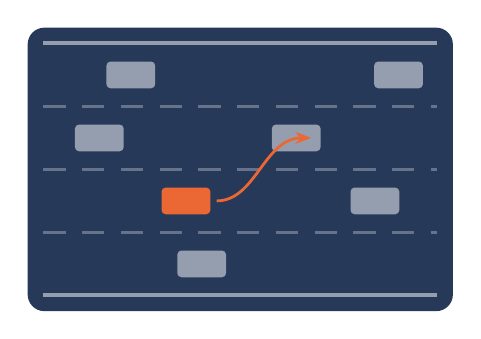
\begin{tikzpicture}[x=1cm,y=1cm]
        \fill[white!8!brand, rounded corners=6pt] (-0.2,-0.2) rectangle (5.2,3.4);
        \foreach \y in {0.8,1.6,2.4} \draw[white!35!brand, line width=1pt, dash pattern=on 8pt off 6pt] (0,\y) -- (5,\y);
        \draw[white!55!brand, line width=1.4pt] (0,0) -- (5,0);
        \draw[white!55!brand, line width=1.4pt] (0,3.2) -- (5,3.2);
        \foreach \x/\y in {0.4/2.0, 2.9/2.0, 1.7/0.4, 3.9/1.2, 4.2/2.8, 0.8/2.8} \fill[white!55!brand, rounded corners=1.5pt] (\x,\y-0.17) rectangle ++(0.62,0.34);
        \fill[accent, rounded corners=1.5pt] (1.5,1.03) rectangle ++(0.62,0.34);
        \draw[accent, line width=1pt, -{Stealth[length=2mm]}] (2.2,1.2) .. controls (2.7,1.2) and (2.8,2.0) .. (3.4,2.0);
      \end{tikzpicture}
    \end{column}
  \end{columns}
  \vfill
\end{darkframe}

\section{Introduction}

\begin{frame}{What We Will See}
  \centering
  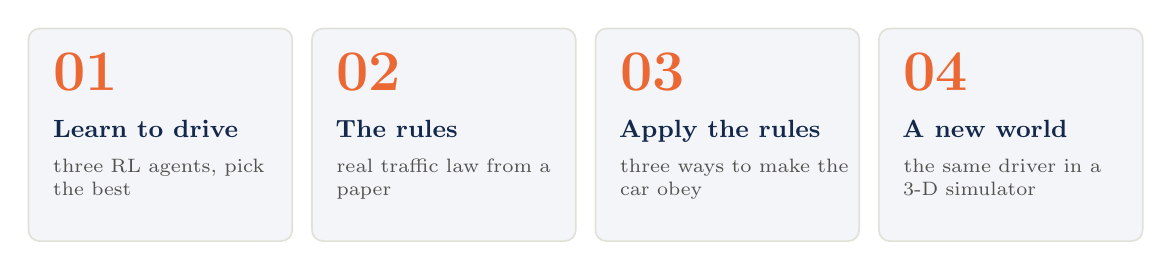
\begin{tikzpicture}
    \foreach \i/\t/\s in {1/Learn to drive/three RL agents{,} pick the best,
                          2/The rules/real traffic law from a paper,
                          3/Apply the rules/three ways to make the car obey,
                          4/A new world/the same driver in a 3-D simulator} {
      \node[card, minimum width=3.35cm, minimum height=2.7cm] (c\i) at ({(\i-1)*3.6},0) {};
      \node[font=\fontsize{22}{22}\selectfont\bfseries, text=accent, anchor=north west] at ($(c\i.north west)+(0.2,-0.2)$) {0\i};
      \node[font=\small\bfseries, text=brand, anchor=north west, text width=2.9cm, align=left] at ($(c\i.north west)+(0.2,-1.05)$) {\t};
      \node[font=\scriptsize, text=ink2, anchor=north west, text width=2.9cm, align=left] at ($(c\i.north west)+(0.2,-1.55)$) {\s};
    }
  \end{tikzpicture}
  \vspace{1.2em}
  \begin{keybox}
    Every rule violation in this talk is counted by an \textbf{independent checker}: never by the reward or the shield
    the car uses. The numbers can be audited.
  \end{keybox}
\end{frame}

\begin{frame}{The Goal: a Fast Brain and a Rulebook}
  \begin{columns}[c]
    \begin{column}{0.46\textwidth}
      \begin{itemize}\small
        \item A \textbf{neural network} learns by itself to overtake traffic, but it drives dangerously and nobody can
              say \emph{why} it acts.
        \item \textbf{Traffic rules} are written by humans: clear and checkable, but they cannot drive.
        \item \textbf{Neuro-Symbolic AI} joins the two: the network drives (System 1, fast), the rules check it
              (System 2, careful).
        \item The same rules then \textbf{explain} every decision: which rule, which fact, which step.
      \end{itemize}
    \end{column}
    \begin{column}{0.5\textwidth}
      \centering
      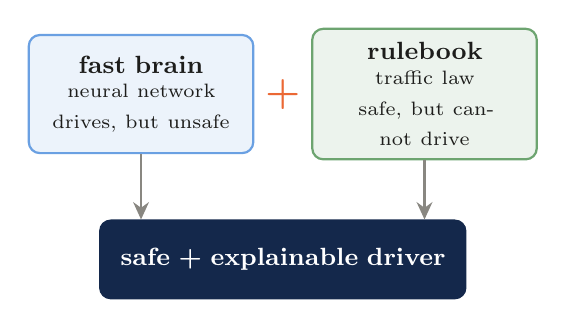
\begin{tikzpicture}
        \node[tint=cblue, text width=2.5cm, minimum height=1.5cm] (nn) at (0,1.9)
          {\textbf{fast brain}\\[0.1em]\scriptsize neural network\\drives, but unsafe};
        \node[tint=softc, text width=2.5cm, minimum height=1.5cm] (rl) at (3.6,1.9)
          {\textbf{rulebook}\\[0.1em]\scriptsize traffic law\\safe, but cannot drive};
        \node[font=\Large\bfseries, text=accent] at (1.8,1.9) {+};
        \node[solid=brand, text width=4.3cm, minimum height=1.0cm] (out) at (1.8,-0.2) {\textbf{safe + explainable driver}};
        \draw[arr] (nn.south) -- (out.north -| nn.south);
        \draw[arr] (rl.south) -- (out.north -| rl.south);
      \end{tikzpicture}
    \end{column}
  \end{columns}
\end{frame}

% ════════════════════════════════════════════════════════════════════════════════════════════════
\partslide{1}{Learn to Drive}{Three reinforcement-learning agents on a busy highway}
\section{Part 1 \,$\cdot$\, Learn to drive}

\begin{frame}{The Highway Environment}
  \centering
  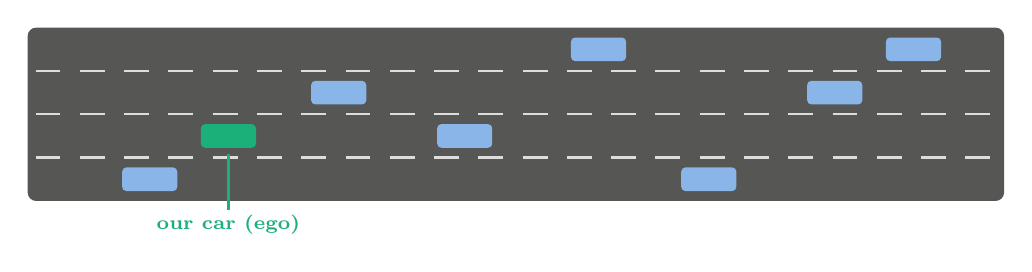
\begin{tikzpicture}[x=1cm,y=1cm]
    \fill[ink!75, rounded corners=3pt] (0,0) rectangle (12.4,2.2);
    \foreach \y in {0.55,1.1,1.65} \draw[white!85!ink, line width=0.8pt, dash pattern=on 9pt off 7pt] (0.1,\y) -- (12.3,\y);
    \foreach \x/\y in {5.2/0.825, 3.6/1.375, 8.3/0.275, 9.9/1.375, 10.9/1.925, 6.9/1.925, 1.2/0.275}
      \fill[cblue!55!white, rounded corners=1.5pt] (\x,\y-0.15) rectangle ++(0.7,0.3);
    \fill[caqua, rounded corners=1.5pt] (2.2,0.675) rectangle ++(0.7,0.3);
    \node[font=\scriptsize\bfseries, text=caqua] at (2.55,-0.3) {our car (ego)};
    \draw[caqua, line width=0.8pt] (2.55,-0.12) -- (2.55,0.6);
  \end{tikzpicture}
  \vspace{0.8em}

  \begin{columns}[T]
    \begin{column}{0.31\textwidth}
      \begin{block}{Sees \normalfont\color{muted}(numbers, not pixels)}
        \footnotesize itself and the 4 nearest cars: present?, position, lane, speeds
      \end{block}
    \end{column}
    \begin{column}{0.31\textwidth}
      \begin{block}{Does \normalfont\color{muted}(2 decisions / s)}
        \footnotesize \texttt{LANE\_LEFT}, \texttt{LANE\_RIGHT}, \texttt{FASTER}, \texttt{SLOWER}, \texttt{IDLE}
      \end{block}
    \end{column}
    \begin{column}{0.31\textwidth}
      \begin{block}{Reward \normalfont\color{muted}(aggressive on purpose)}
        \footnotesize $+$ speed, $+$ each car passed, $-$ one big penalty for a crash
      \end{block}
    \end{column}
  \end{columns}
  \vspace{0.6em}
  {\footnotesize\color{ink2} 4 lanes, 50 cars, 40-second runs. The reward makes a \textbf{fast, risky} driver: exactly
  what the rules must fix later.}
\end{frame}

\begin{frame}{Three Agents, One Fair Test}
  \centering
  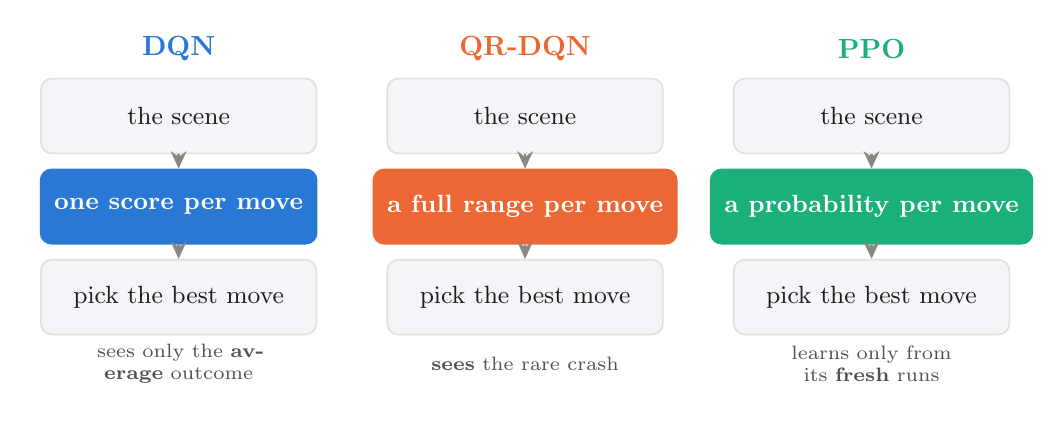
\begin{tikzpicture}[font=\small]
    \foreach \x/\name/\col/\what/\foot [count=\i] in {
        0/DQN/cblue/one score per move/{sees only the \textbf{average} outcome},
        4.4/QR-DQN/accent/a full range per move/{\textbf{sees} the rare crash},
        8.8/PPO/caqua/a probability per move/{learns only from its \textbf{fresh} runs}} {
      \node[font=\normalsize\bfseries, text=\col] at (\x,2.75) {\name};
      \node[card, minimum width=3.5cm] (a\i) at (\x,1.9) {the scene};
      \node[solid=\col, minimum width=3.5cm] (b\i) at (\x,0.75) {\textbf{\what}};
      \node[card, minimum width=3.5cm] (c\i) at (\x,-0.4) {pick the best move};
      \draw[arr] (a\i) -- (b\i);
      \draw[arr] (b\i) -- (c\i);
      \node[lab, text width=3.6cm] at (\x,-1.25) {\foot};
    }
  \end{tikzpicture}
  \vspace{0.3em}
  \begin{itemize}\small
    \item \textbf{DQN} and \textbf{QR-DQN} are twins: QR-DQN only predicts 50 quantiles of the return instead of its mean.
    \item \textbf{Same for all}: road, traffic, reward, 20{,}000 training steps, and the same 50 test runs (10 seeds $\times$ 5).
  \end{itemize}
\end{frame}

\begin{frame}{Learning to Drive}
  \centering
  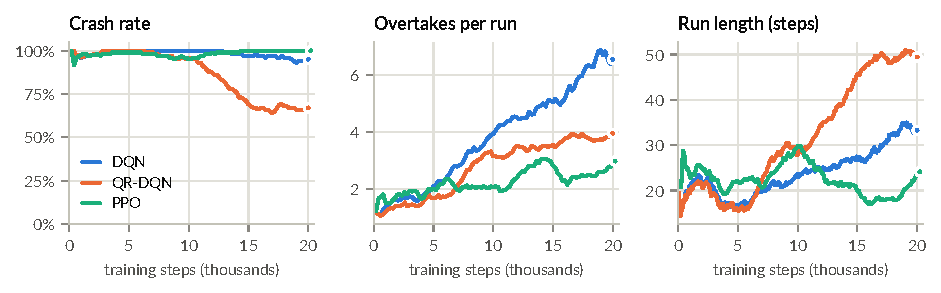
\includegraphics[width=\linewidth]{figures/p1_training.pdf}
  \vspace{0.2em}
  \begin{columns}[T]
    \begin{column}{0.32\textwidth}
      \footnotesize\textcolor{cblue}{\textbf{DQN}} passes the most cars but never stops crashing: the best
      \emph{average} is to drive flat out.
    \end{column}
    \begin{column}{0.32\textwidth}
      \footnotesize\textcolor{accent}{\textbf{QR-DQN}} is the only one whose crashes fall and whose runs get longer:
      it keeps the rare crash in view.
    \end{column}
    \begin{column}{0.32\textwidth}
      \footnotesize\textcolor{caqua}{\textbf{PPO}} learns only from its own fresh runs: 20k steps are not enough.
    \end{column}
  \end{columns}
\end{frame}

\begin{frame}{How the Three Drive}
  \centering
  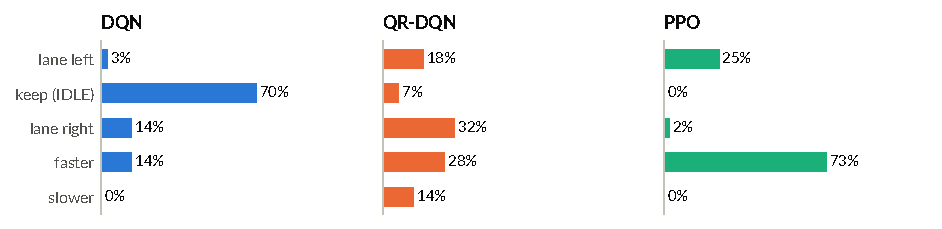
\includegraphics[width=\linewidth]{figures/p1_action_mix.pdf}
  \vspace{0.3em}
  \begin{keybox}
    \textcolor{cblue}{\textbf{DQN}} mostly keeps its lane (70\% \texttt{IDLE}), \textcolor{caqua}{\textbf{PPO}} mostly
    accelerates (73\% \texttt{FASTER}). \textcolor{accent}{\textbf{QR-DQN}} uses all five moves and is the
    \textbf{only one that brakes} (14\% \texttt{SLOWER}): it crashes least.
  \end{keybox}
  {\scriptsize\color{muted} Share of decisions over the same 50 test runs.}
\end{frame}

\begin{frame}{The Final Test: QR-DQN Wins}
  \centering
  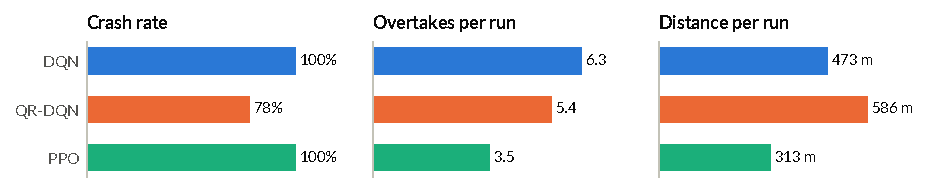
\includegraphics[width=\linewidth]{figures/p1_final_test.pdf}
  \vspace{0.2em}
  \begin{columns}[c]
    \begin{column}{0.56\textwidth}
      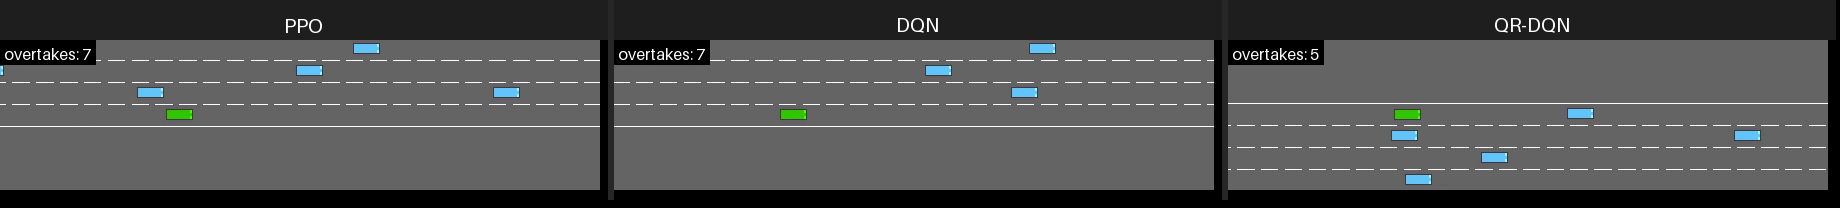
\includegraphics[width=\linewidth]{figures/p1_video_frame.png}
      \par{\scriptsize\color{muted} Best test run of each agent (\texttt{videos/part1\_three\_agents.mp4})}
    \end{column}
    \begin{column}{0.4\textwidth}
      \begin{keybox}
        \textbf{QR-DQN} crashes least and drives furthest. 78\% crashes is still a bad driver, on purpose: that is
        what the rules must fix.
      \end{keybox}
    \end{column}
  \end{columns}
\end{frame}

% ════════════════════════════════════════════════════════════════════════════════════════════════
\partslide{2}{The Rules}{Real traffic law, written as logic}
\section{Part 2 \,$\cdot$\, The rules}

\begin{frame}{Where the Traffic Law Comes From}
  {\footnotesize\color{ink2} S.~Maierhofer et al.\ (TU Munich), \textbf{Formalization of Interstate Traffic Rules in
  Temporal Logic}, IEEE IV 2020}
  \vspace{0.6em}

  \centering
  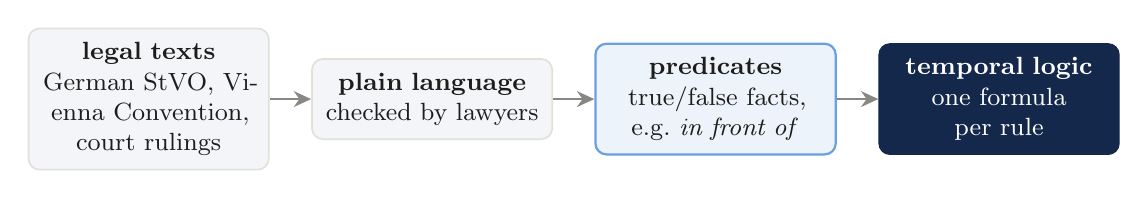
\begin{tikzpicture}[font=\scriptsize]
    \node[card, text width=2.7cm] (a) at (0,0) {\textbf{legal texts}\\German StVO, Vienna Convention, court rulings};
    \node[card, text width=2.7cm] (b) at (3.6,0) {\textbf{plain language}\\checked by lawyers};
    \node[tint=cblue, text width=2.7cm] (c) at (7.2,0) {\textbf{predicates}\\true/false facts, e.g.\ \emph{in front of}};
    \node[solid=brand, text width=2.7cm] (d) at (10.8,0) {\textbf{temporal logic}\\one formula per rule};
    \draw[arr] (a) -- (b); \draw[arr] (b) -- (c); \draw[arr] (c) -- (d);
  \end{tikzpicture}
  \vspace{0.6em}
  \raggedright
  \begin{columns}[T]
    \begin{column}{0.52\textwidth}
      \begin{itemize}\small
        \item \textbf{Metric temporal logic}: logic with time. $\mathbf{G}$ always, $\mathbf{F}$ eventually,
              $\mathbf{P}$ previously, $\mathbf{O}$ once in the past.
        \item Each rule becomes a formula a program can check. RG1, simplified:
      \end{itemize}
      \vspace{-0.2em}
      \[ \mathbf{G}\big(\textit{same lane} \wedge \textit{in front} \wedge \neg\textit{cut-in}\big)
         \Rightarrow \textit{safe distance} \]
    \end{column}
    \begin{column}{0.44\textwidth}
      \begin{block}{Tested on 2,500+ real German drivers}
        \footnotesize
        \begin{itemize}
          \item Only about \textbf{37\%} obey every rule.
          \item Most broken: \textbf{safe distance} ($<$65\% comply) and \textbf{speed limit} ($<$78\%).
          \item Almost nobody stops, brakes for no reason or passes on the right.
        \end{itemize}
      \end{block}
    \end{column}
  \end{columns}
\end{frame}

\begin{frame}{The Six Rules We Use}
  \begin{columns}[T]
    \begin{column}{0.58\textwidth}
      \small
      \renewcommand{\arraystretch}{1.25}
      \begin{tabular}{@{}l l c@{}}
        \toprule
        \textbf{rule} & \textbf{in plain words} & \textbf{kind} \\
        \midrule
        RG1 & keep a safe distance from the car ahead & \hard \\
        RG3 & do not go over the speed limit & \hard \\
        RI1 & do not stop in the middle of the road & \hard \\
        RG2 & do not brake harshly for no reason & \soft \\
        RG4 & do not block the traffic behind you & \soft \\
        RI2 & do not overtake on the right & \soft \\
        \bottomrule
      \end{tabular}
    \end{column}
    \begin{column}{0.38\textwidth}
      \begin{block}{\textcolor{hardc}{Hard}: forbidden}
        \footnotesize Breaking one can directly cause a crash, so the shield \textbf{vetoes} it.
      \end{block}
      \vspace{0.3em}
      \begin{block}{\textcolor{softc}{Soft}: discouraged}
        \footnotesize Bad habits that annoy or slow traffic, so the reward \textbf{penalises} them.
      \end{block}
    \end{column}
  \end{columns}
  \vspace{0.3em}
  \small
  \textbf{Safe distance (RG1)}, from the paper: my reaction and braking distance minus the leader's braking distance.
  \[ d_{\mathrm{safe}} = v_{\mathrm{ego}}\,t_d + \frac{v_{\mathrm{ego}}^2}{2|a_{\mathrm{ego}}|}
                         - \frac{v_{\mathrm{lead}}^2}{2|a_{\mathrm{lead}}|},\qquad
     t_d = 0.3\,\mathrm{s},\ a_{\mathrm{ego}} = -10,\ a_{\mathrm{lead}} = -10.5\ \mathrm{m/s^2} \]
  {\scriptsize\color{ink2} Thresholds: \texttt{configs/highway.yaml} (RG1 from the paper's Table~II).}
\end{frame}

% ════════════════════════════════════════════════════════════════════════════════════════════════
\partslide{3}{Apply the Rules}{Shield, reward shaping and planning on the Part-1 winner (QR-DQN)}
\section{Part 3 \,$\cdot$\, Apply the rules}

\begin{frame}{From the Scene to Facts, from Facts to Actions}
  \centering
  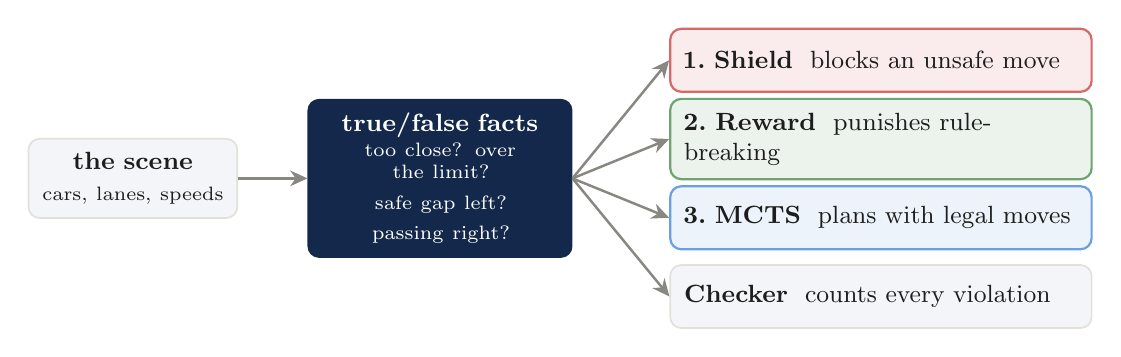
\begin{tikzpicture}[font=\small]
    \node[card, text width=2.3cm] (scene) at (0,0) {\textbf{the scene}\\\scriptsize cars, lanes, speeds};
    \node[solid=brand, text width=3.0cm] (facts) at (3.9,0)
      {\textbf{true/false facts}\\[0.1em]\scriptsize too close? over the limit?\\safe gap left? passing right?};
    \node[tint=hardc, text width=5.0cm, align=left, minimum height=0.8cm] (sh) at (9.5,1.5) {\textbf{1.\ Shield}\ \ blocks an unsafe move};
    \node[tint=softc, text width=5.0cm, align=left, minimum height=0.8cm] (rw) at (9.5,0.5) {\textbf{2.\ Reward}\ \ punishes rule-breaking};
    \node[tint=cblue, text width=5.0cm, align=left, minimum height=0.8cm] (mc) at (9.5,-0.5) {\textbf{3.\ MCTS}\ \ plans with legal moves};
    \node[card, text width=5.0cm, align=left, minimum height=0.8cm] (ck) at (9.5,-1.5) {\textbf{Checker}\ \ counts every violation};
    \draw[arr] (scene) -- (facts);
    \foreach \n in {sh,rw,mc,ck} \draw[arr] (facts.east) -- (\n.west);
  \end{tikzpicture}
  \vspace{0.8em}
  \begin{keybox}
    The facts (\textbf{predicates}) are computed once per step and shared by all three methods \emph{and} the checker:
    one source of truth.
  \end{keybox}
\end{frame}

\begin{frame}{Three Ways to Make the Car Obey}
  \begin{columns}[T]
    \begin{column}{0.32\textwidth}
      \begin{block}{\textcolor{hardc}{Shield} \normalfont\color{muted}(Lab 3)}
        \footnotesize A state machine checks each chosen move. If it breaks a \textbf{hard} rule, it is swapped for the
        safest legal one (brake or keep the lane).\\[0.4em]
        \textcolor{softc}{$+$} no re-training\\\textcolor{hardc}{$-$} cautious, fewer overtakes
      \end{block}
    \end{column}
    \begin{column}{0.32\textwidth}
      \begin{block}{\textcolor{softc}{Reward shaping}}
        \footnotesize A short re-training where each \textbf{soft}-rule violation costs reward (right pass 0.5,
        blocking 0.3, harsh braking 0.3).\\[0.4em]
        \textcolor{softc}{$+$} learns the habit\\\textcolor{hardc}{$-$} no guarantee
      \end{block}
    \end{column}
    \begin{column}{0.32\textwidth}
      \begin{block}{\textcolor{cblue}{MCTS planning} \normalfont\color{muted}(Lab 4)}
        \footnotesize Replaces the network: imagines 20 short futures (3 steps), 70\% of moves drawn from the
        \textbf{legal} ones, and picks the best.\\[0.4em]
        \textcolor{softc}{$+$} rules used \emph{before} acting\\\textcolor{hardc}{$-$} only as good as its model
      \end{block}
    \end{column}
  \end{columns}
  \vspace{0.8em}
  \centering
  {\small Six setups on the same 50 test runs: baseline, $+$shield, $+$logic-reward, $+$shield$+$reward, $+$MCTS,
  $+$MCTS$+$shield.}
\end{frame}

\begin{frame}{Which Method Fixes Which Rule}
  \centering
  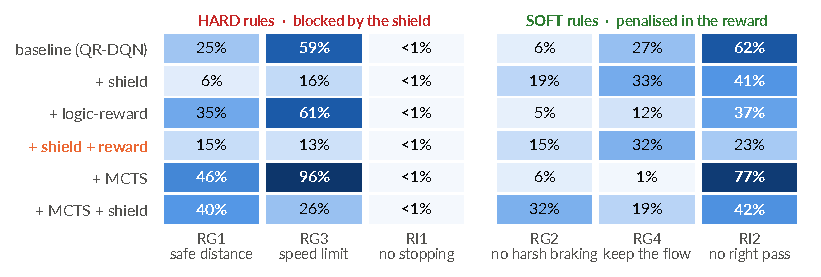
\includegraphics[width=\linewidth]{figures/p2_rule_violations.pdf}
  \par{\scriptsize\color{muted} Share of steps that break each rule (darker = worse), same 50 test runs.}
  \vspace{0.1em}
  \begin{columns}[T]
    \begin{column}{0.24\textwidth}
      \footnotesize\textbf{$+$shield} crushes the \textcolor{hardc}{\textbf{hard}} rules, but brakes more.
    \end{column}
    \begin{column}{0.24\textwidth}
      \footnotesize\textbf{$+$reward} fixes the \textcolor{softc}{\textbf{soft}} rules, but cannot stop speeding.
    \end{column}
    \begin{column}{0.24\textwidth}
      \footnotesize\textcolor{accent}{\textbf{$+$shield$+$reward}}: both low, they fix \textbf{different} rules.
    \end{column}
    \begin{column}{0.24\textwidth}
      \footnotesize\textbf{$+$MCTS} plans for speed: it speeds and passes right the most.
    \end{column}
  \end{columns}
\end{frame}

\begin{frame}{Putting It Together: Shield + Reward Wins}
  \begin{columns}[c]
    \begin{column}{0.6\textwidth}
      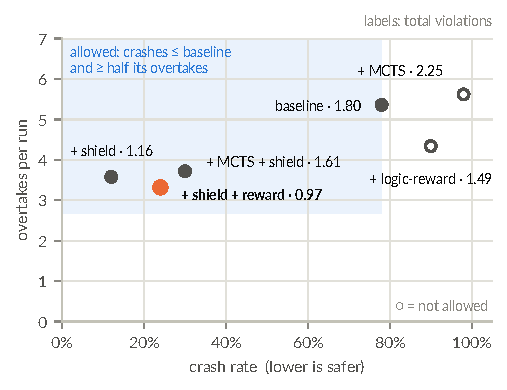
\includegraphics[width=\linewidth]{figures/p2_tradeoff.pdf}
    \end{column}
    \begin{column}{0.38\textwidth}
      \footnotesize
      \begin{itemize}
        \item \textbf{Allowed} (blue area): crashes no more than the baseline \textbf{and} at least half its overtakes.
        \item Among the allowed setups, the \textbf{fewest violations} wins: \textcolor{accent}{\textbf{shield $+$
              reward}} (0.97, from 1.80).
        \item \textbf{Violations} = the six per-rule rates added up.
      \end{itemize}
      \begin{keybox}
        The shield alone is the safest: crashes \textbf{78\% $\to$ 12\%}, with no re-training at all.
      \end{keybox}
    \end{column}
  \end{columns}
\end{frame}

\begin{frame}{Six Setups on the Same Road}
  \centering
  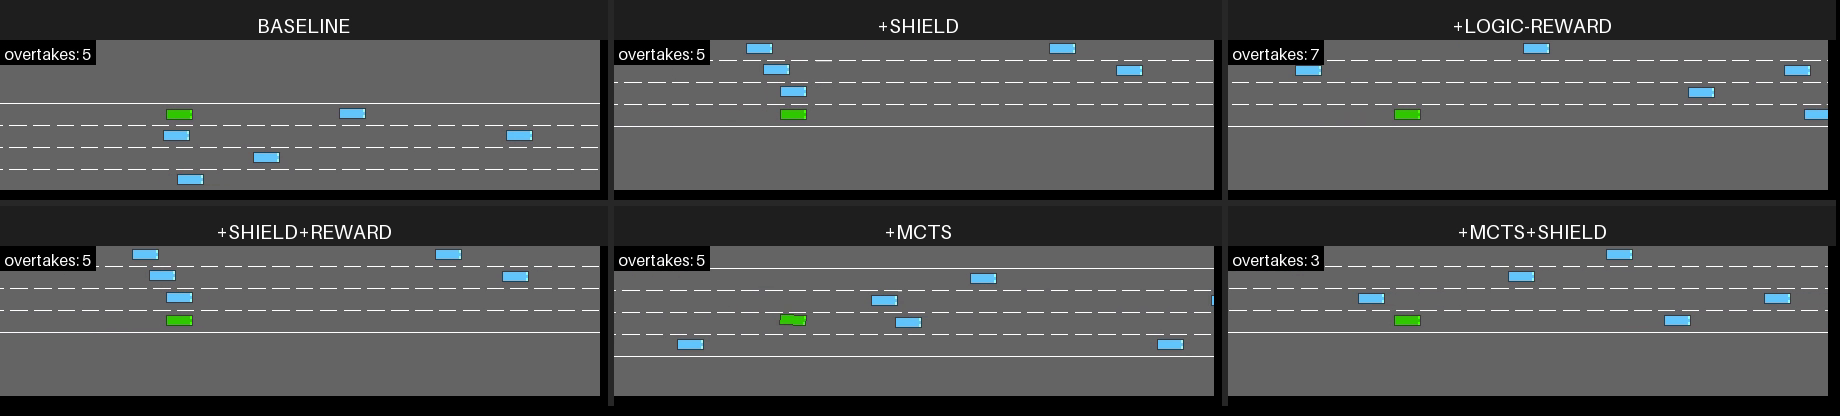
\includegraphics[width=0.94\linewidth]{figures/p2_video_frame.png}
  \par{\scriptsize\color{muted} Best test run of each setup (\texttt{videos/part2\_six\_setups.mp4}). Green = our car.}
  \vspace{0.8em}
  \begin{keybox}
    With the shield the car changes lane less and passes fewer cars, but it crashes far less.
  \end{keybox}
\end{frame}

% ════════════════════════════════════════════════════════════════════════════════════════════════
\partslide{4}{A New World}{The same driver and the same rules in MetaDrive, a 3-D robot simulator}
\section{Part 4 \,$\cdot$\, A new world}

\begin{frame}{The Same Driver, a New Simulator}
  \centering
  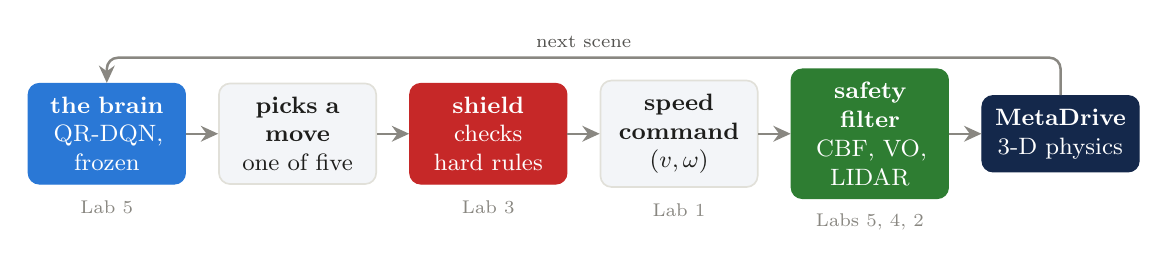
\begin{tikzpicture}[font=\scriptsize, scale=0.95, every node/.style={transform shape}]
    \node[solid=cblue, text width=1.75cm] (b) at (0,0) {\textbf{the brain}\\QR-DQN, frozen};
    \node[card, text width=1.75cm] (m) at (2.55,0) {\textbf{picks a move}\\one of five};
    \node[solid=hardc, text width=1.75cm] (s) at (5.1,0) {\textbf{shield}\\checks hard rules};
    \node[card, text width=1.75cm] (c) at (7.65,0) {\textbf{speed command}\\$(v,\omega)$};
    \node[solid=softc, text width=1.75cm] (f) at (10.2,0) {\textbf{safety filter}\\CBF, VO, LIDAR};
    \node[solid=brand, text width=1.75cm] (w) at (12.75,0) {\textbf{MetaDrive}\\3-D physics};
    \foreach \p/\q in {b/m, m/s, s/c, c/f, f/w} \draw[arr] (\p) -- (\q);
    \foreach \n/\l in {b/Lab 5, s/Lab 3, c/Lab 1, f/{Labs 5, 4, 2}} \node[lab, text=muted] at ($(\n.south)+(0,-0.3)$) {\l};
    \draw[arr, rounded corners] (w.north) -- ++(0,0.5) -| node[lab, above, pos=0.25] {next scene} (b.north);
  \end{tikzpicture}
  \vspace{0.6em}
  \begin{columns}[T]
    \begin{column}{0.5\textwidth}
      \begin{block}{Everything changes except the rules}
        \footnotesize Other physics, 3 lanes instead of 4, starts from 0 m/s, robot-scale speeds ($\approx$9 m/s).
        The network \textbf{never trained here}.
      \end{block}
    \end{column}
    \begin{column}{0.46\textwidth}
      \begin{block}{The safety filter}
        \footnotesize \textbf{CBF} keeps the gap and speed, \textbf{VO} blocks unsafe steering, \textbf{LIDAR} brakes for
        close cars in front.
      \end{block}
    \end{column}
  \end{columns}
  \vspace{0.4em}
  {\footnotesize\color{ink2} Question: does the safety come from the \textbf{rules} or from the \textbf{network}? Three setups,
  20 runs each on a $\approx$650 m road.}
\end{frame}

\begin{frame}{One Rule, Three Encodings}
  \centering
  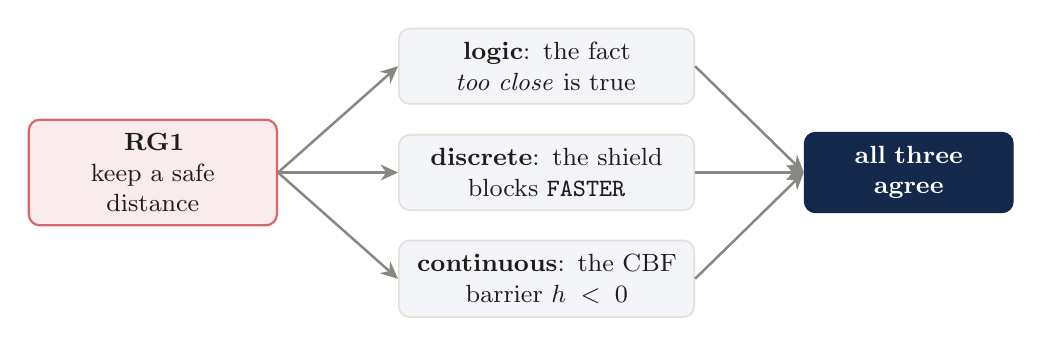
\begin{tikzpicture}[font=\small]
    \node[tint=hardc, text width=2.8cm] (r) at (0,0) {\textbf{RG1}\\keep a safe distance};
    \node[card, text width=3.4cm] (a) at (5.0,1.35) {\textbf{logic}: the fact\\\emph{too close} is true};
    \node[card, text width=3.4cm] (b) at (5.0,0) {\textbf{discrete}: the shield\\blocks \texttt{FASTER}};
    \node[card, text width=3.4cm] (c) at (5.0,-1.35) {\textbf{continuous}: the CBF\\barrier $h<0$};
    \node[solid=brand, text width=2.3cm] (ok) at (9.6,0) {\textbf{all three agree}};
    \foreach \n in {a,b,c} { \draw[arr] (r.east) -- (\n.west); \draw[arr] (\n.east) -- (ok.west); }
  \end{tikzpicture}
  \vspace{1.0em}
  \begin{keybox}
    The same safe-distance rule, written three ways. A check (\texttt{rule\_encoding\_agreement}) confirms they
    \textbf{always agree}: the rule survived the move to a new world unchanged.
  \end{keybox}
\end{frame}

\begin{frame}{Same Rules, New World}
  \centering
  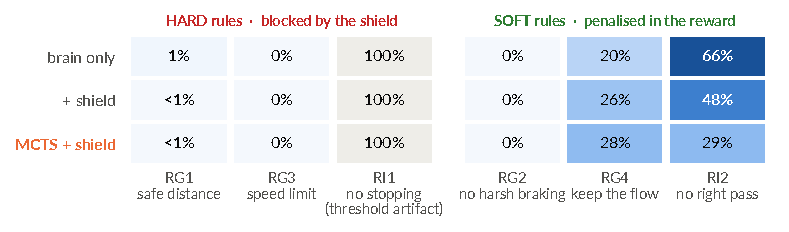
\includegraphics[width=\linewidth]{figures/p3_rule_violations.pdf}
  \vspace{0.4em}
  \begin{columns}[T]
    \begin{column}{0.32\textwidth}
      \footnotesize\textbf{Hard rules solved.} The CBF enforces safe distance and speed at every step.
    \end{column}
    \begin{column}{0.32\textwidth}
      \footnotesize\textbf{Dense traffic.} A car often on the left means right passes (RI2) and slow flow (RG4);
      \textbf{MCTS} breaks the fewest.
    \end{column}
    \begin{column}{0.32\textwidth}
      \footnotesize\textbf{RI1 is not a real failure.} ``Stopped'' means below 18 m/s, set for the highway; the robot
      drives at $\approx$8 m/s.
    \end{column}
  \end{columns}
\end{frame}

\begin{frame}{Which Setup Wins Here?}
  \centering
  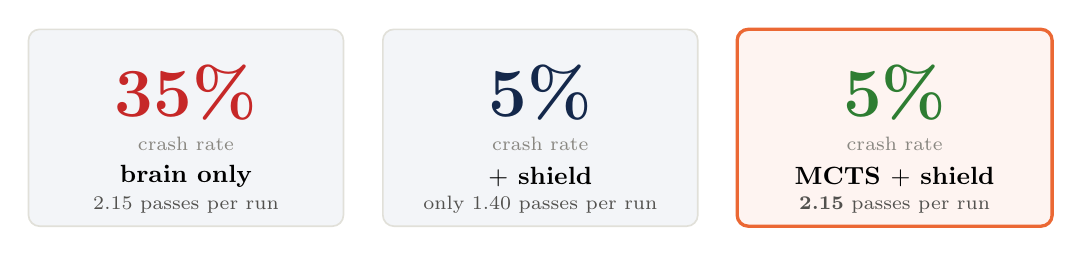
\begin{tikzpicture}
    \foreach \x/\num/\col/\name/\sub/\fill in {
        0/35\%/hardc/brain only/{2.15 passes per run}/surface,
        4.5/5\%/brand/$+$ shield/{only 1.40 passes per run}/surface,
        9.0/5\%/softc/MCTS $+$ shield/{\textbf{2.15} passes per run}/accent!7} {
      \node[card, fill=\fill, minimum width=4.0cm, minimum height=2.5cm] at (\x,0) {};
      \node[font=\fontsize{30}{30}\selectfont\bfseries, text=\col] at (\x,0.45) {\num};
      \node[font=\scriptsize, text=muted] at (\x,-0.2) {crash rate};
      \node[font=\small\bfseries] at (\x,-0.62) {\name};
      \node[font=\scriptsize, text=ink2] at (\x,-0.98) {\sub};
    }
    \draw[accent, line width=1.2pt, rounded corners=4pt] (7.0,-1.25) rectangle (11.0,1.25);
  \end{tikzpicture}
  \vspace{0.8em}
  \begin{keybox}
    \textbf{Why MCTS wins:} the shield alone is safe but too cautious. MCTS plans on the \textbf{real} scene, so a new world
    does not confuse it, and it uses the rules \textbf{before} acting. The shield keeps it safe; MCTS gives back the overtaking.
  \end{keybox}
\end{frame}

\begin{frame}{In Motion}
  \begin{columns}[T]
    \begin{column}{0.32\textwidth}
      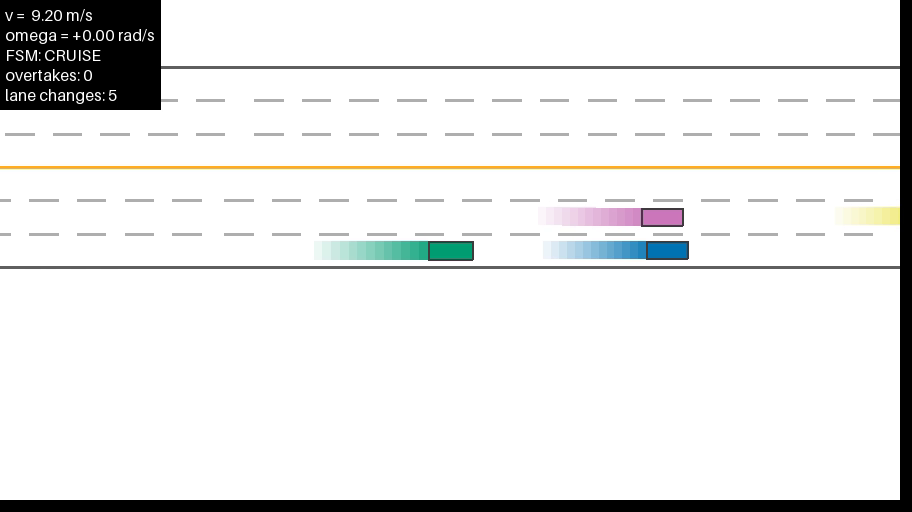
\includegraphics[width=\linewidth]{figures/p3_brain_only_frame.png}
      \par\centering{\scriptsize\textcolor{hardc}{\textbf{brain only}}: crashes}
    \end{column}
    \begin{column}{0.32\textwidth}
      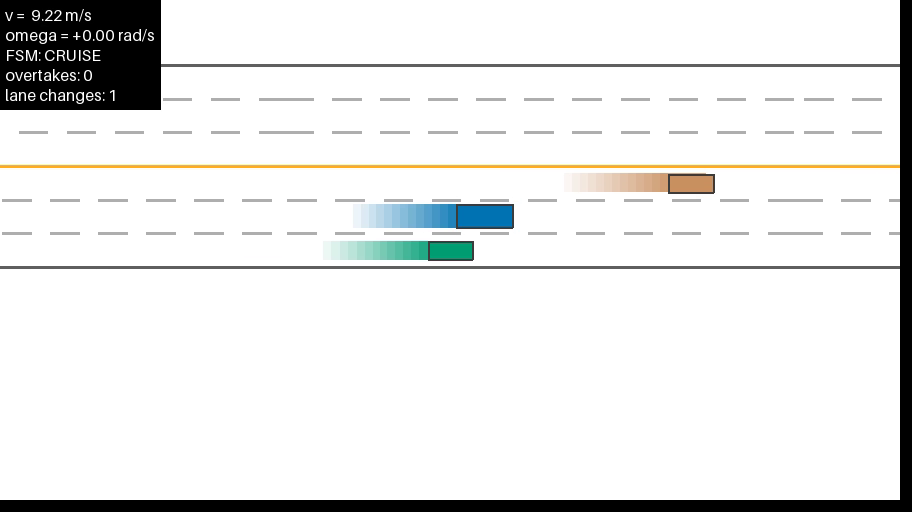
\includegraphics[width=\linewidth]{figures/p3_shield_frame.png}
      \par\centering{\scriptsize\textbf{$+$ shield}: safe}
    \end{column}
    \begin{column}{0.32\textwidth}
      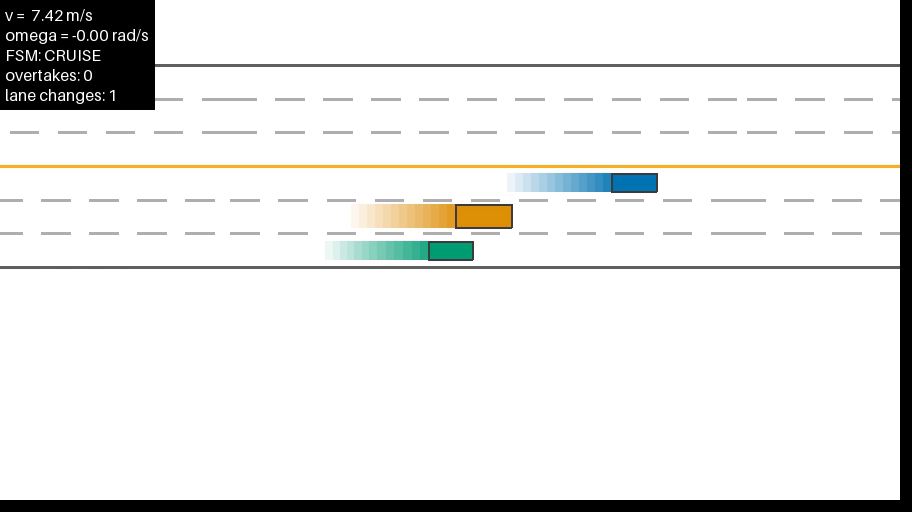
\includegraphics[width=\linewidth]{figures/p3_mcts_shield_frame.png}
      \par\centering{\scriptsize\textcolor{softc}{\textbf{MCTS $+$ shield}}: safe and passes}
    \end{column}
  \end{columns}
  \vspace{0.5em}
  \begin{columns}[c]
    \begin{column}{0.38\textwidth}
      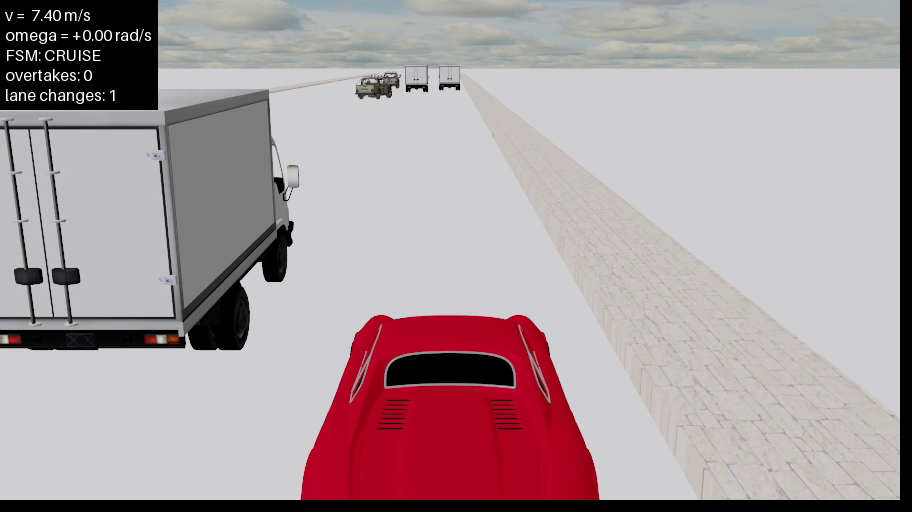
\includegraphics[width=\linewidth]{figures/p3_winner_3d_frame.png}
    \end{column}
    \begin{column}{0.58\textwidth}
      \footnotesize
      \begin{itemize}
        \item Top: each setup's best run, from above. Green = our car.
        \item Left: the winner in the 3-D chase view; the panel shows the speed command $(v,\omega)$, the shield's
              state and the overtakes.
        \item All clips: \texttt{videos/} next to this file.
      \end{itemize}
    \end{column}
  \end{columns}
\end{frame}

% ════════════════════════════════════════════════════════════════════════════════════════════════
\section{Conclusion}

\begin{frame}{Hard Rules With the Shield: Lower, Not Zero}
  \begin{columns}[c]
    \begin{column}{0.54\textwidth}
      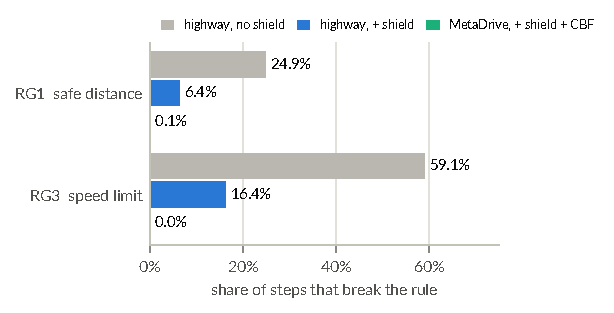
\includegraphics[width=\linewidth]{figures/hard_rules_shield.pdf}
    \end{column}
    \begin{column}{0.43\textwidth}
      \small
      \begin{itemize}
        \item On the highway the shield cuts \textbf{RG1} from 25\% to 6.4\% of steps and \textbf{RG3} from 59\% to
              16.4\%, but not to zero.
        \item In MetaDrive, shield $+$ \textbf{CBF} brings both to $\approx$0.
      \end{itemize}
      \begin{keybox}
        To find out why, we \textbf{replayed the same 50 test runs} and logged, at every violating step, what the shield
        saw and what it did. The replay matches the saved results exactly.
      \end{keybox}
    \end{column}
  \end{columns}
\end{frame}

\begin{frame}{Why: the Shield Is Reactive}
  \centering
  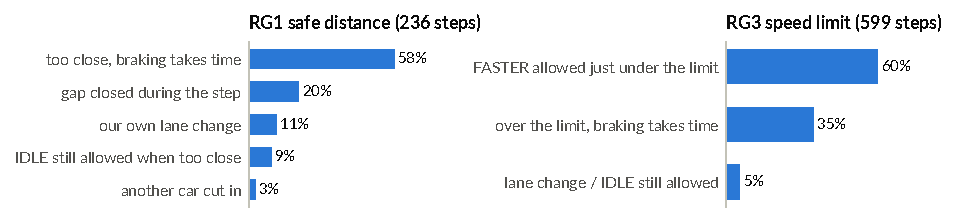
\includegraphics[width=\linewidth]{figures/shield_causes.pdf}
  \par{\scriptsize\color{muted} Cause of every violating step in the replay of the $+$shield test runs.}
  \vspace{0.3em}
  \begin{columns}[T]
    \begin{column}{0.32\textwidth}
      \footnotesize\textbf{Acts only after the fact.} It brakes once the rule is broken; speed changes gradually
      ($\approx$0.6 s), so the gap reopens slowly.
    \end{column}
    \begin{column}{0.32\textwidth}
      \footnotesize\textbf{Checks now, not next.} \texttt{FASTER} below 25 m/s sets the target to 30 m/s: the car
      overshoots.
    \end{column}
    \begin{column}{0.32\textwidth}
      \footnotesize\textbf{Small gaps in the mask.} \texttt{IDLE} allowed when too close. Cut-ins: only 3\%.
    \end{column}
  \end{columns}
  \vspace{0.3em}
  \begin{keybox}
    \textbf{Fix:} a \textbf{predictive} shield that checks the state \emph{after} the move, like the CBF in MetaDrive
    ($\approx$0).
  \end{keybox}
\end{frame}

\begin{frame}{What We Learned}
  \begin{columns}[T]
    \begin{column}{0.55\textwidth}
      \begin{block}{Lessons}
        \footnotesize
        \begin{itemize}
          \item The network alone drives fast but crashes: \textbf{a reward is not enough}.
          \item A \textbf{shield} makes it safe with no re-training (78\% $\to$ 12\% crashes).
          \item A \textbf{shaped reward} teaches habits but gives no guarantee.
          \item Shield and reward fix \textbf{different} rules: together, the fewest violations.
          \item \textbf{MCTS $+$ shield} was safe \emph{and} overtaking in a world it never trained on.
          \item The same rules worked in \textbf{two simulators}, checked by an independent monitor.
        \end{itemize}
      \end{block}
    \end{column}
    \begin{column}{0.41\textwidth}
      \begin{block}{Limits}
        \footnotesize
        \begin{itemize}
          \item Short training (20k steps): the best driver still crashes in 78\% of runs.
          \item Small tests: 50 runs on the highway, 20 in MetaDrive.
          \item Highway thresholds make RI1 and RI2 read too high on the robot.
          \item The highway shield is reactive; the CBF is a simple version (no QP).
        \end{itemize}
      \end{block}
    \end{column}
  \end{columns}
\end{frame}

\begin{frame}{What Comes Next: Intersection Rules}
  \begin{columns}[T]
    \begin{column}{0.55\textwidth}
      {\footnotesize\color{ink2} S.~Maierhofer et al., \textbf{Formalization of Intersection Traffic Rules in Temporal
      Logic}, IEEE IV 2022}
      \vspace{0.5em}
      \begin{itemize}\small
        \item The same method for junctions: traffic lights, stop and give-way signs, unregulated crossings.
        \item Stop at red lights and stop signs, give way to the right, yield to oncoming cars when turning left.
        \item Split into hard and soft rules, like the highway rules.
      \end{itemize}
    \end{column}
    \begin{column}{0.41\textwidth}
      \begin{keybox}
        \textbf{The plan:} merge both papers into \textbf{one rule set} and switch rules with the place. The
        \textbf{same driver} then works safely in many worlds just by loading the right rules.
      \end{keybox}
    \end{column}
  \end{columns}
\end{frame}

\begin{darkframe}
  \vfill
  \hspace*{0.9cm}\begin{minipage}{0.8\textwidth}
    {\color{white}\fontsize{30}{34}\selectfont\bfseries Thank you\par}
    \vspace{0.8em}
    {\color{accent}\rule{2.4cm}{2pt}}\par\vspace{0.8em}
    {\color{white!75!brand}\small \presenter\ \,$\cdot$\, \studentid}
  \end{minipage}
  \vfill
\end{darkframe}

\end{document}
